\chapter{Método do trabalho} \label{cap:metodo}


Este capítulo apresenta o método adotado na construção da proposta deste trabalho. A definição da solução foi conduzida a partir de três frentes complementares: levantamento bibliográfico, análise técnica das tecnologias envolvidas e organização da arquitetura do sistema. O objetivo desse processo foi estruturar uma proposta coerente para comunicação, segurança e análise de dados em um cenário de sistemas embarcados e Internet das Coisas.

Inicialmente, é apresentada a arquitetura de comunicação e infraestrutura do sistema, que estabelece o caminho de coleta, encaminhamento e armazenamento dos dados. Em seguida, são apresentadas as etapas relacionadas à segurança e ao uso de aprendizado de máquina, consideradas como partes integradas à solução proposta. Ao final, o capítulo organiza os elementos que orientam a implementação e a avaliação do sistema.

%%%%%%%%%%%%%%%%%%%%%%%%%%%%%%%%%%%%%%%%%%%%%%%%%%%%
%%%%%%%%%%%%%%%%%%%%%%%%%%%%%%%%%%%%%%%%%%%%%%%%%%%%

\section{Procedimento de definição da arquitetura do sistema}

A definição da arquitetura do sistema foi conduzida a partir da combinação entre levantamento bibliográfico, análise técnica das tecnologias envolvidas e separação em módulos da solução proposta. O objetivo dessa etapa foi estruturar uma arquitetura coerente com o problema estudado, considerando as restrições típicas de sistemas embarcados, a necessidade de comunicação em campo e a integração posterior com mecanismos de segurança e análise.

Como referência metodológica para essa definição, o trabalho adota princípios inspirados no modelo RM-ODP, utilizando diferentes pontos de vista para organizar a solução. Em termos funcionais, foram identificados os principais blocos responsáveis pela coleta, encaminhamento, recebimento e armazenamento das informações. Em termos de informação, foram considerados os dados de aplicação e os metadados necessários para rastreabilidade, segurança e análise posterior. Em termos de engenharia, foram observadas as separações entre o trecho embarcado da comunicação, o gateway e a infraestrutura de backend.

A partir dessa organização, a arquitetura foi estruturada de modo a separar claramente a comunicação em campo da camada de aplicação. Essa separação permite tratar, de forma independente, as restrições energéticas dos nós sensores, o papel intermediário do gateway e as funções de autenticação, persistência e análise associadas ao backend. Com isso, a definição arquitetural deixa de ser apenas uma escolha de componentes e passa a refletir a distribuição de responsabilidades entre as partes do sistema.

Além da decomposição dos componentes, o procedimento de definição da arquitetura também considerou o fluxo das informações ao longo da solução. Para isso, foram analisadas as interações entre os nós de campo, o gateway e a infraestrutura de backend, buscando garantir que o sistema fosse capaz de receber, registrar e armazenar dados e metadados de forma compatível com as etapas posteriores do trabalho.

Por fim, a representação da interação entre os principais componentes foi organizada também por meio de diagramas, de modo a tornar mais clara a sequência de eventos envolvida na coleta, no encaminhamento e no armazenamento das mensagens. Essa modelagem auxilia tanto na compreensão da proposta quanto na transição entre a etapa metodológica e a etapa posterior de especificação da arquitetura.

\subsection{Critérios adotados na decomposição arquitetural}

A modularização da arquitetura foi orientada por três critérios principais. O primeiro foi a separação entre o trecho de comunicação em campo e a infraestrutura de aplicação, de modo a preservar as vantagens do uso de LoRa no nível embarcado e da comunicação baseada em rede IP no nível de backend. O segundo foi a definição de responsabilidades distintas para coleta, encaminhamento, autenticação e persistência, evitando concentrar funções heterogêneas em um único componente. O terceiro foi a necessidade de manter a solução compatível com a incorporação posterior de mecanismos de criptografia leve e análise por aprendizado de máquina.

Esses critérios levaram à definição de uma arquitetura em blocos com papéis bem delimitados. No trecho embarcado, concentram-se as funções de aquisição e transmissão inicial dos dados. No ponto de transição, o gateway atua como elemento de integração entre a rede de campo e a infraestrutura de aplicação. No backend, concentram-se as funções de autenticação, persistência e preparação dos dados para uso posterior. Essa divisão favorece clareza arquitetural, reduz acoplamento entre responsabilidades e facilita a evolução incremental da solução.

\subsection{Modelagem das interações e do fluxo de dados}

Para explicitar a dinâmica de funcionamento da proposta, o fluxo principal de interação entre os componentes foi modelado em termos de sequência de eventos. Essa modelagem considera a coleta dos dados no nó de campo, a transmissão pelo enlace LoRa ponto a ponto, a recepção e o enriquecimento da mensagem no gateway, o encaminhamento ao backend por Wi-Fi e HTTP, e o armazenamento final de dados e metadados na infraestrutura de persistência.

A utilização de um diagrama de sequência nessa etapa é importante porque permite representar, de forma mais direta, a ordem das interações entre os componentes e os pontos em que ocorre o tratamento das mensagens. Com isso, o fluxo deixa de ser apenas uma descrição textual e passa a ser apresentado também como uma sequência organizada de ações entre entidades bem definidas.

\begin{figure}[htb]
  \caption{\label{infra_arch_1}Diagrama de sequência UML do fluxo principal}
  \begin{center}
      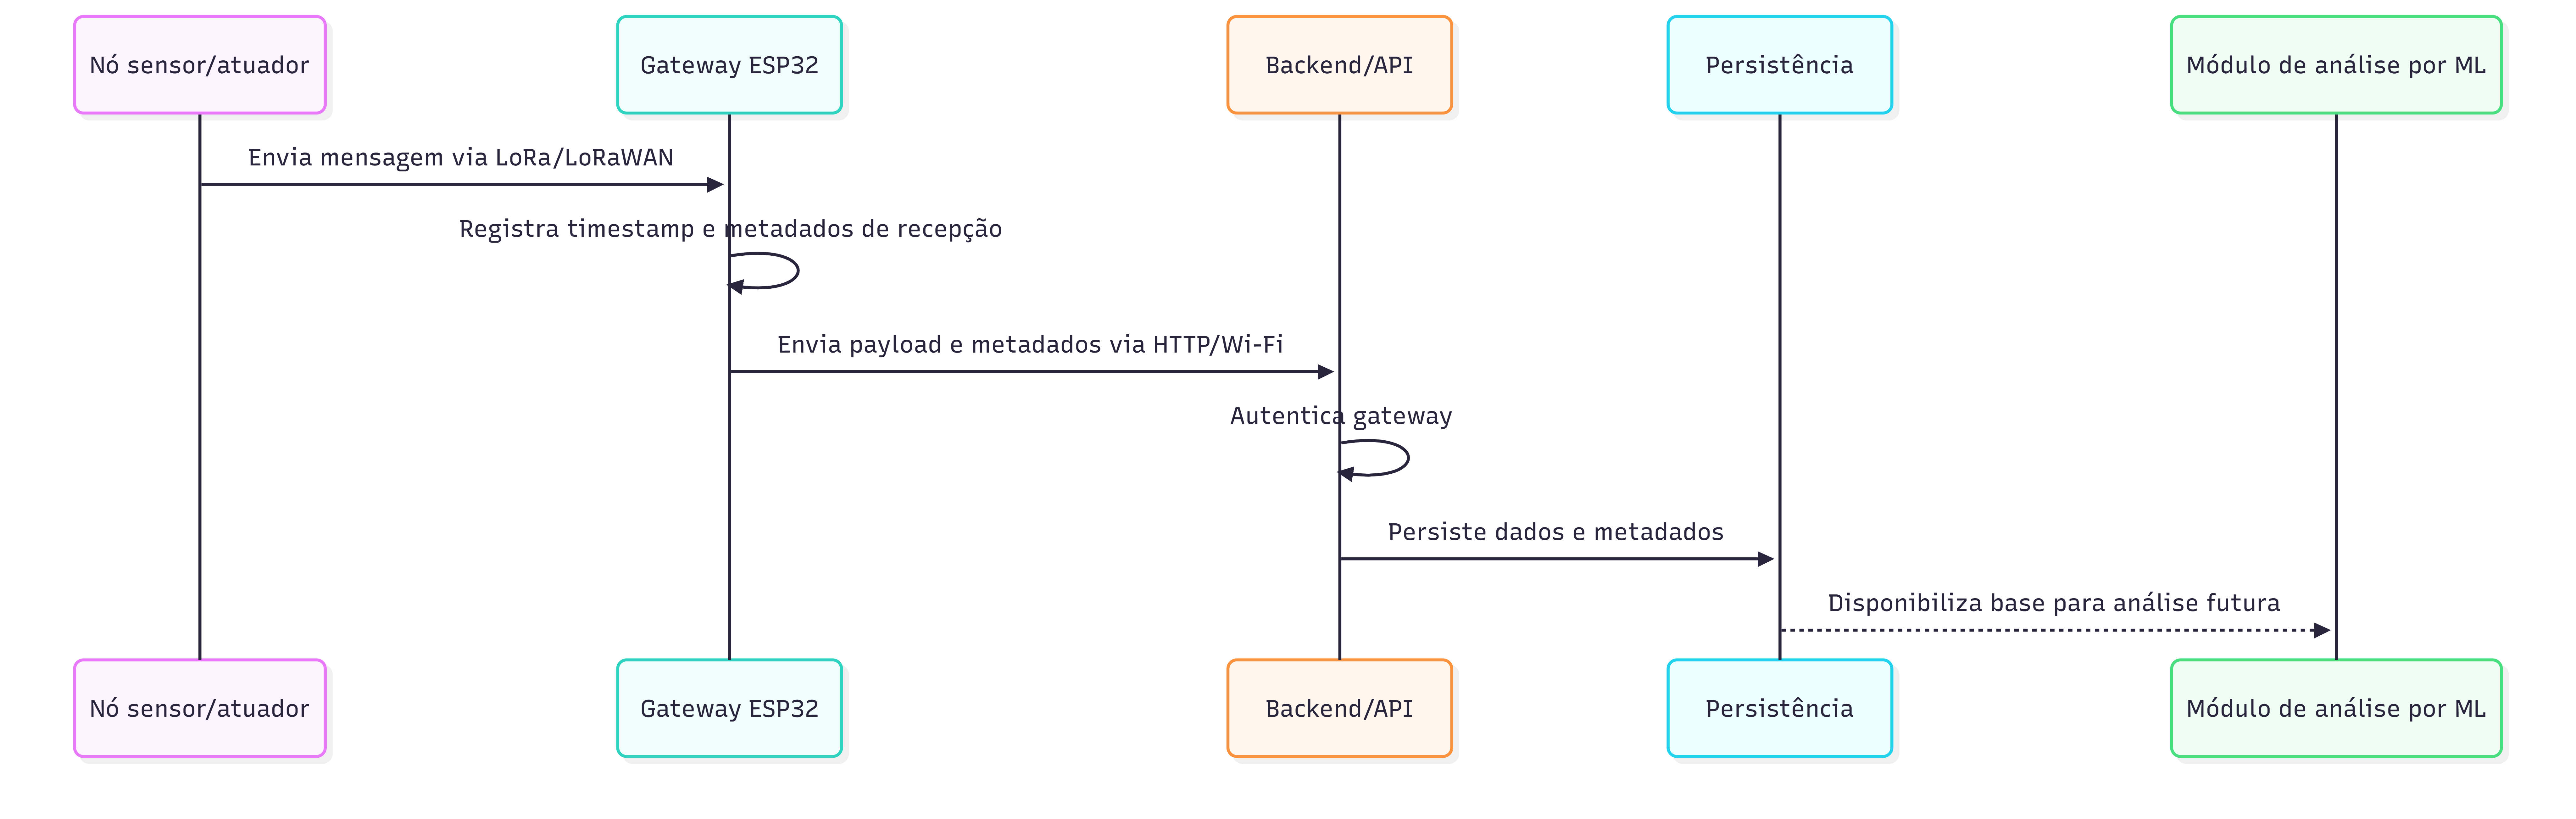
\includegraphics[scale=0.05]{barea/figuras/arch-2-uml.png}
  \end{center}

\end{figure}

Essa representação também ajuda a evidenciar que o sistema foi concebido para operar de forma orientada a evento. Em vez de depender de comunicação contínua, o fluxo é ativado pela geração e recepção das mensagens produzidas em campo, o que torna a proposta mais compatível com o tipo de aplicação e com as restrições energéticas associadas aos dispositivos embarcados.

%%%%%%%%%%%%%%%%%%%%%%%%%%%%%%%%%%%%%%%%%%%%%%%%%%%%
%%%%%%%%%%%%%%%%%%%%%%%%%%%%%%%%%%%%%%%%%%%%%%%%%%%%


\section{Especificação de Requisitos e Revisão Bibliográfica}

%%%%%%%%%%%%%%%%%%%%%%%%%%%%%%%%%%%%%%%%%%%%%%%%%%%%
\subsection{Materiais e bases de dados}
\label{subsec:ml-dataset}

Esta parte do método trata do modelo de detecção. Ela parte do RSSI, o
metadado de recepção definido na Seção~\ref{subsec:camada_fisica_lora}, e
entrega o detector que o \textit{gateway} da Seção~\ref{sec:requisitos_infra}
executa, descrito na Seção~\ref{subsec:ml-protocolo-borda}. O modelo é estimado
com o \textit{dataset} Tour Perret,
publicado pelo CampusIoT da Université Grenoble Alpes \cite{tourperret_dataset}.
Ele reúne os eventos de cinco nós sensores instalados na Tour Perret, em
Grenoble, recebidos de 25/06/2021 a 23/06/2023 por um servidor de rede
ChirpStack v3, num total de 421.937 mensagens. O arquivo usado é o oficial,
conferido pelo resumo SHA-256 publicado com ele. Cada evento de
\textit{uplink} traz uma lista com uma entrada por \textit{gateway} que recebeu
o quadro, com o RSSI medido naquele \textit{gateway} \cite{brocaarintegration}.

O \textit{dataset} vem de sensores em operação real e não tem rótulos de ataque.
Por isso ele serve para aprender o comportamento esperado do RSSI, e a
capacidade de detecção é medida com desvios sintéticos, como descrito na
Seção~\ref{subsec:ml-protocolo-deteccao}.

\subsection{Limpeza e recorte da série}
\label{subsec:ml-limpeza}
% sec:selecao_variaveis: rótulo citado pelas Seções 2.1 e 3.1 (barea); aqui se define que o modelo usa só o RSSI.
\label{sec:selecao_variaveis}

A limpeza segue regras numeradas, cada uma com a contagem de linhas depois de
aplicada, como mostram a Tabela~\ref{tab:ml-limpeza} e a
Figura~\ref{fig:ml-funil}. Os dados ficam em duas tabelas, uma de quadros e
outra de recepções, segundo o princípio de uma linha por observação
\cite{wickham2014tidy}. As regras têm quatro papéis diferentes. L1 e L4 removem
registros que não são medidas novas. L2 e L3 só organizam os dados. L6 e L8 não
removem dados inválidos. Elas fazem o recorte do estudo, escolhendo um nó
sensor e um trecho contínuo. L7 e L9 apenas marcam quadros, sem remover nada, e
L5 registra a decisão de não filtrar o RSSI.

\begin{table}[htb]
	\centering
	\caption{Regras de limpeza e recorte da série de RSSI}
	\label{tab:ml-limpeza}
	\begin{tabular}{llr}
		\hline
		\textbf{Regra} & \textbf{O que faz} & \textbf{Linhas depois} \\
		\hline
		L1 & Mantém só eventos de \textit{uplink} & 421.906 \\
		L2 & Usa o instante de arquivamento como eixo de tempo & 421.906 \\
		L3 & Separa quadros e recepções (recepções) & 3.559.119 \\
		L4 & Remove retransmissões (quadros) & 398.699 \\
		L5 & Não aplica limite físico ao RSSI & 398.699 \\
		L6 & Seleciona o nó sensor \texttt{441a1ed9} & 193.442 \\
		L7 & Marca trocas de taxa de dados e quedas do FCnt & 193.442 \\
		L8 & Seleciona o maior trecho sem lacuna maior que 1~h & 58.540 \\
		L9 & Marca os quadros sem RSSI no \textit{gateway} escolhido & 58.540 \\
		\hline
	\end{tabular}
	\legend{Fonte: elaborado pelos autores.}
\end{table}

\begin{figure}[htb]
	\centering
	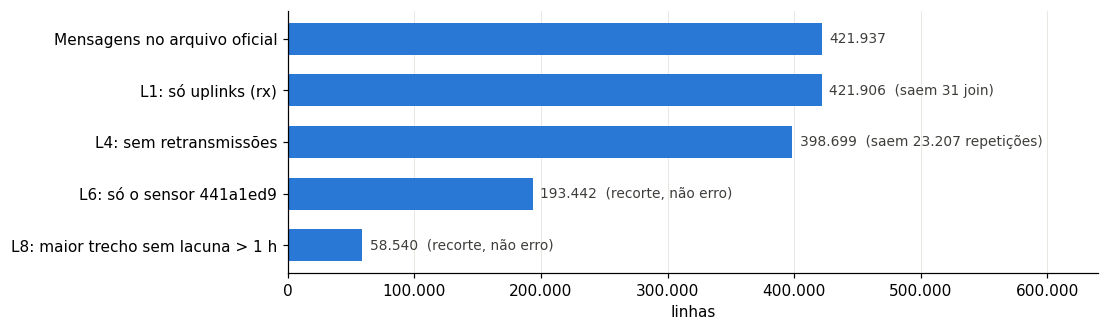
\includegraphics[width=0.85\textwidth]{tadaki/figuras/ml-funil-limpeza.png}
	\caption{Quantidade de linhas depois de cada etapa da limpeza e do recorte}
	\label{fig:ml-funil}
	\legend{Fonte: elaborado pelos autores.}
\end{figure}

A regra L4 trata como retransmissão o quadro do mesmo nó sensor com o mesmo
FCnt do anterior, recebido em menos de 60~s, porque o FCnt não sobe quando o
mesmo quadro é reenviado \cite{lorawan103}. No trecho usado, a janela de 60~s
não muda nada, pois de 10~s a sem limite são sempre as mesmas 4
retransmissões. A regra L5 deixa o RSSI sem filtro, porque no trecho usado ele
fica entre $-120$ e $-90$~dBm e um valor extremo pode trazer informação sobre o
processo \cite{hyndman2021}, que é justamente o que a detecção procura.

O estudo usa só o RSSI, de um nó sensor e de um \textit{gateway}. Entre os cinco
nós sensores, o \texttt{441a1ed9} tem ao mesmo tempo o maior número de quadros
(193.442), a taxa de dados mais estável (99,99\% em DR5, com 13 trocas) e o
maior trecho contínuo (58.540 quadros, contra no máximo 24.992 dos outros). O
\textit{gateway} \texttt{17459c66} é o de maior cobertura desse nó sensor, com
97,2\% dos quadros. O maior trecho sem intervalo acima de 3.600~s vai de
16/11/2021 a 08/06/2022, em 203,7 dias, e é o mesmo para qualquer limite entre
3.600 e 14.400~s.

\subsection{Preparação da série}
\label{subsec:ml-preparacao}

Depois da limpeza, quatro decisões transformam os quadros em uma série pronta
para o modelo. A série começa no primeiro quadro com RSSI observado, porque
antes dele não há valor anterior a repetir, o que descarta 4 quadros e deixa
58.536. O quadro que o \textit{gateway} escolhido não recebeu, 2,8\% do
trecho, recebe o último valor observado e fica marcado. Essa forma de
preencher usa só o passado. Uma alternativa medida, deixar o vazio para o
próprio modelo tratar, mudou o RMSE de validação do ARIMA por canal de
1,136 para 1,135~dBm.

O eixo da série é a ordem dos quadros, e não o relógio, porque o modelo supõe
passos iguais. O nó sensor transmite a intervalos regulares. O intervalo entre
quadros consecutivos tem mediana de 300,0~s e fica até 300,03~s em 99\% dos
casos, e só 24 dos 58.535 intervalos passam de 600~s. A divisão é cronológica,
como mostra a Tabela~\ref{tab:ml-divisao}.

\begin{table}[htb]
	\centering
	\caption{Divisão da série em treino, validação e teste}
	\label{tab:ml-divisao}
	\begin{tabular}{lrlr}
		\hline
		\textbf{Parte} & \textbf{Quadros} & \textbf{Período (UTC)} & \textbf{Sem RSSI} \\
		\hline
		Treino (70\%) & 40.975 & 16/11/2021 a 08/04/2022 & 1.355 \\
		Validação (15\%) & 8.780 & 08/04/2022 a 08/05/2022 & 121 \\
		Teste (15\%) & 8.781 & 08/05/2022 a 08/06/2022 & 138 \\
		\hline
	\end{tabular}
	\legend{Fonte: elaborado pelos autores.}
\end{table}

O treino estima os coeficientes do modelo. A validação serve a todas as
escolhas, a ordem do modelo e o limiar do alarme. O teste é usado uma única vez
para cada configuração final.

\subsection{Protocolo de avaliação da previsão}
\label{subsec:ml-protocolo}

Toda previsão é um passo à frente. Os coeficientes do ARIMA são estimados uma
vez no treino e depois aplicados, fixos, ao resto da série
\cite{statsmodelsapply}, de modo que cada quadro é previsto com os valores
reais até o quadro anterior, como faria o \textit{gateway}. A diferenciação é
decidida pelo teste KPSS no treino, a ordem é escolhida pelo RMSE na validação,
e cada configuração final é avaliada uma única vez no teste.

O erro é medido pelo RMSE e pelo MAE da Seção~\ref{subsec:ml-avaliacao} e
também pela mediana do erro absoluto, que indica o erro típico de um quadro.
As três medidas usam só os quadros com RSSI observado, porque num quadro
preenchido o \textit{random walk} acerta por construção.

O modelo é comparado com duas referências. A primeira é o \textit{random walk}
da Equação~\ref{eq:ml-random-walk}. A segunda, mais exigente, é o
\textit{random walk} por canal, que repete o último valor observado no mesmo
canal de frequência. Ganhar desta segunda referência mostra que o modelo
acrescenta algo além de separar os canais.

A robustez dos resultados é verificada de quatro formas. O mesmo procedimento é
repetido no \textit{gateway} \texttt{100210b9}. A ordem do modelo é variada um
parâmetro de cada vez, para ver se o resultado depende de uma ordem
específica. A execução completa, do \textit{dataset} bruto aos resultados, é
refeita numa cópia isolada do projeto. Por fim, para medir quanto dado de
treino basta, o ARIMA é estimado com treinos de 6~h a 142 dias, todos
terminando no fim do treino e avaliados na mesma validação. Um tamanho basta
quando o RMSE fica abaixo do \textit{random walk} por canal e no máximo 20\%
acima do obtido com o treino inteiro.

\subsection{Protocolo da detecção}
\label{subsec:ml-protocolo-deteccao}

A detecção usa a regra da Equação~\ref{eq:ml-deteccao} sobre o erro do modelo
final. Em cada canal, o limiar $\tau$ é o quantil de 99\% do erro absoluto na
validação, o que fixa cerca de 1\% de alarmes falsos sem depender da suposição
de normalidade \cite{hundman2018spacecraft}. O limiar nunca fica abaixo de
1,5~dB, porque o \textit{gateway} informa o RSSI em valores inteiros de dB.

Como o \textit{dataset} não tem ataques identificados, a detecção é medida com
desvios sintéticos, somados a uma cópia do teste. Cada desvio é um degrau de
$+\Delta$ ou $-\Delta$~dB, com $\Delta$ de 1 a 10~dB, em dois formatos, um de 12
quadros, cerca de 1~h, e outro de um só quadro. O sentido positivo segue o
efeito do \textit{jamming} reativo sobre o RSSI \cite{ruotsalainen2022jamming}.
Cada combinação é aplicada em 300 posições sorteadas do teste, uma de cada vez,
com semente fixa, e o valor alterado entra no histórico do modelo, como
aconteceria na borda. As medidas são a taxa de alarmes falsos no teste sem
desvio e a fração dos desvios com ao menos um alarme, com intervalo de
confiança de 95\% pelo método de Wilson.

Para saber quanto da detecção vem do modelo, o mesmo protocolo é aplicado a um
detector mais simples, que usa como previsão o \textit{random walk} por canal.
Como o RSSI é inteiro, o erro desse detector também é inteiro, e o limiar por
quantil não consegue fixar o alarme falso em 1\%. Por isso ele é avaliado em
duas versões. A primeira usa a mesma regra, o que dá menos alarmes falsos que o
ARIMA, e a segunda usa o limiar um valor inteiro abaixo, o que dá mais.

\subsection{Execução do detector no microcontrolador}
\label{subsec:ml-protocolo-borda}

Com os coeficientes fixos, a previsão um passo à frente do ARIMA$(0,1,1)$ é a
suavização exponencial simples \cite{hyndman2021}, como na
Equação~\ref{eq:ml-borda}, em que $\alpha = 1 + \theta$ e $\theta$ é o
coeficiente de média móvel estimado no treino de cada canal.
\begin{equation}
	\hat{y}_{t+1} = \hat{y}_t + \alpha \left( y_t - \hat{y}_t \right)
	\label{eq:ml-borda}
\end{equation}

Por isso o detector não precisa de biblioteca de séries temporais. Para cada
canal ele guarda $\alpha$, o limiar e a última previsão. Esses valores são
exportados do Python para um arquivo de cabeçalho em C++, e o mesmo código é
compilado para o computador e para a placa Heltec WiFi LoRa 32 V3, com ESP32-S3,
usada pela frente de infraestrutura. A conferência compara, quadro a quadro,
a previsão e o alarme do detector com os do Python, na série de teste e na mesma
série com um desvio sintético de $+5$~dB por 12 quadros. No \textit{gateway} do
protótipo, o detector roda depois do registro de cada quadro autenticado, sem
alterar o dado registrado, e um botão da placa soma um desvio sintético ao RSSI
que o detector recebe, para simular um ataque.



\subsection{Biblioteca Ascon}
\label{subsec:biblioteca-ascon}
Para a implementação das primitivas criptográficas no microcontrolador, optou-se pela utilização da biblioteca de código aberto \textit{ascon-suite}, mantida por \citeonline{weatherley2023ascon}. A escolha desta implementação específica, em detrimento do repositório de referência matemático original (\textit{ascon-c}), justifica-se por fatores arquiteturais estritamente alinhados aos objetivos de prototipagem em sistemas embarcados.

Primeiramente, a \textit{ascon-suite} foi estruturada com foco em plataformas com restrição de recursos, fornecendo rotinas de \textit{backend} altamente otimizadas em linguagem \textit{Assembly}, podendo ser usada diretamente na IDE do Arduino como uma biblioteca, facilitando o desenvolvimento na placa ESP32.

Em segundo lugar, a biblioteca expõe, além da interface de uma única chamada, uma API incremental que permite cifrar mensagens em fragmentos sucessivos, mantendo apenas o estado interno de 80 bytes entre as chamadas. Esse recurso não é exigido pelos \textit{payloads} deste trabalho, que cabem integralmente em memória, mas amplia a margem de crescimento da solução para mensagens maiores que a RAM disponível.

Por fim, o rigor técnico da biblioteca possui forte validação científica. Os códigos otimizados em \textit{Assembly} e C que deram origem à \textit{ascon-suite} foram empregados como base metodológica para a extração de métricas de desempenho em microcontroladores durante o processo de padronização do NIST, com resultados documentados na seção 4.1.3 do relatório oficial NIST IR 8454 \cite{nistir8454}. Uma das três plataformas de teste ali utilizadas é o ESP32 (Xtensa LX6, 240~MHz), o mesmo microcontrolador e a mesma frequência adotados neste trabalho.

A implementação utilizada neste trabalho, fornecida pela biblioteca ascon-suite, corresponde à versão finalista submetida à competição de Criptografia Leve do NIST (Ascon v1.2), e não à forma normatizada posteriormente na publicação SP 800-232 (2025). Especificamente, adota-se a variante Ascon-128a, que compartilha a mesma estrutura de permutação do Ascon-AEAD128 padronizado. As diferenças entre a v1.2 e o SP 800-232 concentram-se no vetor de inicialização, na ordenação de bytes na interface de entrada/saída e na separação de domínio. Como o custo computacional do Ascon é dominado pelas aplicações da permutação, idênticas nas duas versões, espera-se que as métricas de desempenho, memória e energia sejam essencialmente equivalentes.

%%%%%%%%%%%%%%%%%%%%%%%%%%%%%%%%%%%%%%%%%%%%%%%%%%%%
%%%%%%%%%%%%%%%%%%%%%%%%%%%%%%%%%%%%%%%%%%%%%%%%%%%%


\section{Testes e Avaliação de Desempenho (\textit{Benchmarking})}
\label{subsec:validacao-ascon}
\subsection{\textit{Known Answer Tests} (KAT)}
A primeira etapa é a validação através dos \textit{Known Answer Tests} (KAT), que são testes disponibilizados pelo próprio grupo que desenvolveu o Ascon. Eles fornecem parâmetros de entrada específicos que devem resultar em saídas exatas e já esperadas. Como o trabalho utiliza a variante Ascon-128a (versão 1.2), a validação emprega os vetores de teste correspondentes a essa versão, distribuídos junto à própria \textit{ascon-suite} e derivados do repositório de referência \textit{ascon-c} \cite{ascon_reference_c}.

Para validar a biblioteca de forma puramente matemática, os testes são rodados exaustivamente em um computador desktop. Depois, para garantir que não haja nenhuma anomalia de compilação ou diferença causada pela arquitetura de hardware, testes adicionais são executados diretamente na placa, com um volume menor de vetores.

Como garantia extra, a validação na placa precede qualquer coleta de desempenho, de modo que as medições incidam apenas sobre uma implementação já verificada, o próprio \textit{firmware} de medição repete dois vetores do KAT, e um vetor de referência do AES-GCM, antes de medir, e interrompe a execução se algum deles falhar. Ao comparar as saídas das funções da biblioteca \textit{ascon-suite} com os resultados oficiais, comprova-se de forma prática que a implementação opera corretamente no ambiente do projeto.

%%%%%%%%%%%%%%%%%%%%%%%%%%%%%%%%%%%%%%%%%%%%%%%%%%%%

\subsection{Validação dos Dados Associados (AEAD)}
Outro teste é a validação da autenticidade do modo AEAD e a sua capacidade de rejeição de anomalias. Para avaliar a resiliência do sistema contra um ataque de \textit{Man-in-the-middle} (MitM), no qual um interceptador tenta forjar ou corromper a mensagem em trânsito, a metodologia emprega a técnica de injeção intencional de falhas (\textit{bit-flipping}).

Após a geração de um pacote válido, o firmware de teste altera intencionalmente bits específicos antes de repassar a mensagem para a função de decifragem. A adulteração é testada em três frentes distintas.
\begin{itemize}
\item \textbf{No texto cifrado (\textit{Ciphertext}):} simulando um atacante que tenta alterar o valor do \textit{payload} do sensor.
\item \textbf{Nos Dados Associados (AD):} alterando o cabeçalho do protocolo LoRaWAN, simulando uma tentativa de modificar metadados de roteamento ou de identificação do nó.
\item \textbf{Na \textit{Tag} de Autenticação:} simulando um cenário onde a mensagem é modificada e o atacante anexa uma assinatura forjada ou corrompida.
\end{itemize}

O resultado esperado em todos os cenários de adulteração é que a função de decifragem do algoritmo reconheça a quebra de integridade e falhe imediatamente, retornando um código de erro e garantindo que nenhum fragmento do texto claro modificado seja entregue para a camada de aplicação do microcontrolador.

%%%%%%%%%%%%%%%%%%%%%%%%%%%%%%%%%%%%%%%%%%%%%%%%%%%%

\subsection{Vazamento de Memória e Ataques de Canal Colateral}
A avaliação de desempenho não se limita à validação funcional e engloba também o consumo de memória (RAM) e o tempo de execução. Para a análise de memória, a metodologia emprega as funções nativas do ESP-IDF. O uso do \textit{Heap} é monitorado por meio da função \texttt{esp\_get\_free\_heap\_size()} antes e depois da execução e, durante a execução, por uma tarefa no segundo núcleo do processador que lê o \textit{heap} livre continuamente e registra o menor valor observado, de modo a detectar alocações feitas e liberadas dentro da própria operação, invisíveis à comparação entre o antes e o depois. Adicionalmente, mede-se a profundidade máxima alcançada na Pilha (\textit{Stack}) através da função \texttt{uxTaskGetStackHighWaterMark()}, lida dentro de uma tarefa dedicada à operação, uma vez que essa marca registra o ponto mais fundo já atingido pela pilha da tarefa, lida na tarefa principal ela refletiria o uso anterior de outras rotinas, e não o do algoritmo.

Outro aspecto avaliado é o espaço ocupado de memória. O procedimento consiste em compilar o firmware e analisar o uso de memória Flash, comparando os resultados do compilador com e sem a inclusão da biblioteca no projeto.

Quanto ao tempo de execução, a metodologia busca não apenas medir a eficiência, mas também validar a resistência das implementações contra ataques de canal colateral baseados em tempo (\textit{Timing Side-Channel Attacks}). A medição extrai diretamente a quantidade de ciclos de \textit{clock} processados, lendo o contador de ciclos da CPU do ESP32 por meio da função \texttt{ESP.getCycleCount()}, para a cifragem e para a decifragem, em \textit{payloads} de 0, 2, 16, 23, 32 e 64 bytes. Os múltiplos de 16 bytes sustentam o modelo linear de custo por bloco, o \textit{payload} vazio mede a parcela fixa diretamente, e 2 e 23 bytes correspondem aos dois tamanhos de mensagem que ocorrem no \textit{dataset} Tour Perret, usado pela frente de aprendizado de máquina. Em cada tamanho é tomado o piso, o menor valor de 2.000 medidas, com as interrupções habilitadas, de modo que Ascon e AES sejam medidos exatamente da mesma forma. O \textit{driver} de AES do ESP-IDF já protege a operação de bloco com uma seção crítica própria \cite{espressif2026idf}, e o piso de 2.000 medidas faz o papel de filtro contra as interrupções que atingem o restante da chamada. Para o Ascon, o piso com as interrupções desabilitadas é medido como contraprova. Para validar a mitigação de ataques de canal colateral, são realizados testes repetitivos enviando cargas de dados (\textit{payloads}) com conteúdos e chaves completamente distintos, mas de tamanhos idênticos, incluindo classes de entrada fixas (todos os bytes nulos, todos 0xFF, alternados) e variáveis (rampa e valores derivados de um \textit{hash}), na linha do método dudect, que compara o tempo entre classes de entrada em vez de confiar numa única distribuição \cite{reparaz2017dudect}. O resultado esperado é que a variação nos ciclos de \textit{clock} consumidos seja desprezível, coerente com o projeto do algoritmo. A camada de substituição do Ascon dispensa tabelas de consulta, o que afasta ataques de temporização por cache \cite{ascon_v12_spec}. Dessa forma, o tempo de processamento do nó sensor não permite ao atacante deduzir fragmentos da chave ou da mensagem.

Por fim, para verificar a reprodutibilidade, o procedimento é repetido em 100 execuções independentes por tamanho de \textit{payload}, registrando-se o piso de ciclos (o menor valor medido) de cada execução, nas duas placas do projeto, o ESP32 clássico e o ESP32-S3 da placa Heltec com LoRa. A análise distingue a variação entre execuções, dada pela dispersão dos pisos, da variação interna a cada execução, dada pelo desvio padrão de suas medidas. O mesmo se aplica ao comparativo com o AES-128-GCM, tomando como métrica a razão entre os pisos, que cancela fatores comuns às duas medições.

%%%%%%%%%%%%%%%%%%%%%%%%%%%%%%%%%%%%%%%%%%%%%%%%%%%%

\subsection{Avaliação de Consumo Energético}
\label{subsec:energia_metodo}
A avaliação restringe-se ao custo energético das operações criptográficas, não incluindo o consumo da transmissão via rádio. A medição é realizada através da técnica de monitoramento da queda de tensão em um resistor de precisão (\textit{shunt}) de 1$\Omega$ conectado em série com a alimentação de 3,3V do microcontrolador \cite{hubble2024esp32power}, conforme a Figura~\ref{fig_setup_consumo}. As capturas são feitas com um osciloscópio digital, utilizando um pino GPIO como sinal de gatilho (\textit{trigger}) para delimitar com precisão o intervalo de tempo exato da execução das funções criptográficas.

Considerando que o módulo \textit{ESP32 DevKitV1} possui componentes periféricos que consomem corrente de forma constante, como o LED de operação, o regulador de tensão LDO e o conversor USB-Serial, a análise não foca no consumo absoluto da placa. Em vez disso, é aplicada a metodologia de Diferença de Consumo ($\Delta$), na qual subtrai-se a corrente de repouso (\textit{baseline}) do sistema ocioso do valor obtido durante o processamento do algoritmo.

Uma operação isolada não é mensurável dessa forma. A cifragem de 23 bytes dura cerca de 27~$\mu$s, e um acréscimo de poucos miliampères nesse intervalo desaparece no ruído da corrente de repouso da placa, da ordem de 50~mA, com a resolução de 8 bits do osciloscópio. Por isso cada operação é repetida 20.000 vezes em sequência, com o pino de gatilho em nível alto durante toda a rajada, que dura de meio segundo a dois segundos conforme o algoritmo e a placa. O osciloscópio registra a rajada inteira, e toma-se a média da tensão no resistor dentro da janela da rajada e a média em um trecho de repouso da mesma captura. A diferença entre as duas, dividida pela resistência, é a corrente que a operação acrescenta, e a energia por operação é o produto da tensão na placa, desse acréscimo e da duração da rajada, dividido pelo número de repetições. Além do Ascon-128a e do AES-128-GCM, em cifragem e decifragem, mede-se um caso de controle em que o processador apenas aguarda o mesmo tempo em um laço, para separar o custo de manter o núcleo ativo do custo do algoritmo. Durante a medição a placa é alimentada apenas pela fonte, com o cabo USB desconectado, porque o regulador da placa e o terra do cabo criariam caminhos de corrente por fora do resistor.

\begin{figure}[htb]
  \caption{\label{fig_setup_consumo}Configuração de medição de corrente via resistor \textit{shunt} e osciloscópio}
  \begin{center}
      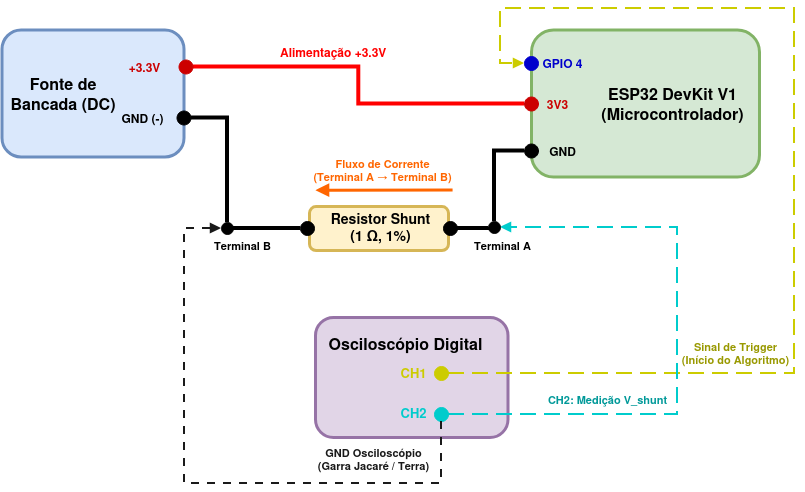
\includegraphics[scale=0.5]{felipe/figuras/setup_consumo_energia.png}
  \end{center}
  \legend{Fonte: Elaborado pelos autores (2026) com base em \cite{hubble2024esp32power}}
\end{figure}

